\documentclass[12pt, a4paper]{article}
\usepackage[margin = 1in, top=1.3in]{geometry}
\usepackage[english]{babel}
\usepackage[utf8]{inputenc}
\usepackage{fancyhdr}
\usepackage[fleqn]{amsmath}
\usepackage{mathtools}
\usepackage{tabto}
\usepackage{bm}
\usepackage{graphicx}
\graphicspath{{./images/}}
\usepackage[font=small,labelfont=bf]{caption}
 
\usepackage{listings}
\usepackage{xcolor}

\definecolor{codegreen}{rgb}{0,0.6,0}
\definecolor{codegray}{rgb}{0.5,0.5,0.5}
\definecolor{codepurple}{rgb}{0.58,0,0.82}
\definecolor{backcolour}{rgb}{0.95,0.95,0.92}

\lstdefinestyle{mystyle}{
    backgroundcolor=\color{backcolour},   
    commentstyle=\color{codegreen},
    keywordstyle=\color{magenta},
    numberstyle=\tiny\color{codegray},
    stringstyle=\color{codepurple},
    basicstyle=\ttfamily\footnotesize,
    breakatwhitespace=false,         
    breaklines=true,                 
    captionpos=b,                    
    keepspaces=true,                 
    numbers=left,                    
    numbersep=5pt,                  
    showspaces=false,                
    showstringspaces=false,
    showtabs=false,                  
    tabsize=2
}

\lstset{style=mystyle}  
 
\pagestyle{fancy}
\fancyhf{}
\rhead{\small{Shaan Ul Haque(180070053)\\ Samarth Singh (180050090) \\ Niraj Mahajan (180050069)}}
\lhead{CS-663 Assignment-5 : Question 5}
\rfoot{Page 5.\thepage}
 
\begin{document}
\vspace*{-22pt}
\section*{Question 5}
\subsection*{1. Code}
\begin{lstlisting}[language=Matlab]
function [x,y, impulse, visibility] = getTranslation(I1,I2)
    [r1,c1] = size(I1);
    [r2,c2] = size(I2);
    assert(r1 == r2);
    assert(c1 == c2);
    
    % calculate FFTs
    F1 = fft2(I1);
    F2 = fft2(I2);
    
    % compute the cross-power spectrum, and the corresponding impulse
    Prod = (F1.*conj(F2))./(abs(F1.*F2) + 1e-15);
    prod = abs(ifft2(Prod));
    impulse = prod/max(prod(:));
    
    % interpret the translation from the obtained impulse
    [~, linearIndexesOfMaxes] = max(prod(:));
    y = rem(linearIndexesOfMaxes-1,300);
    x = (linearIndexesOfMaxes-y-1)/300;
    startx = x;
    starty = y;
    if (x > idivide(int32(c1),2))
       x = x - c1;
    end
    if (y > idivide(int32(r1),2))
       y = y - r1;
    end
    
    % create a yellow circle around the impulse for better visibility
    visibility = cat(3,impulse,impulse,impulse);
    visibility = visibility/max(visibility(:));
    circle = zeros(20,20,3);
    for i = 1:20
        for j = 1:20
            if (abs((i-10)^2 + (j-10)^2 - 81) < 20)
                circle(i,j,:) = [1,1,0];
            end
        end
    end
    visibility(starty-9:starty+10, startx-9:startx+10,:) = visibility(starty-9:starty+10, startx-9:startx+10,:) + circle;
end
\end{lstlisting}
\newpage
\subsection*{2. Image Registration without noise}
In the noiseless case, the translation was obtained at $t_x = -30$ and $t_y = 70$. \\
Below are the corresponding plots. The 4th plot is just the 3rd plot with a marking circle added for better visibility. (Kindly zoom-in the pdf for better clarity)
\vspace*{65pt}
\begin{figure}[h!]
    \centering
    \renewcommand{\thefigure}{5.1}
    \begin{minipage}[c][1\width]{0.7\textwidth}
    	\hspace*{-0.8in}
    	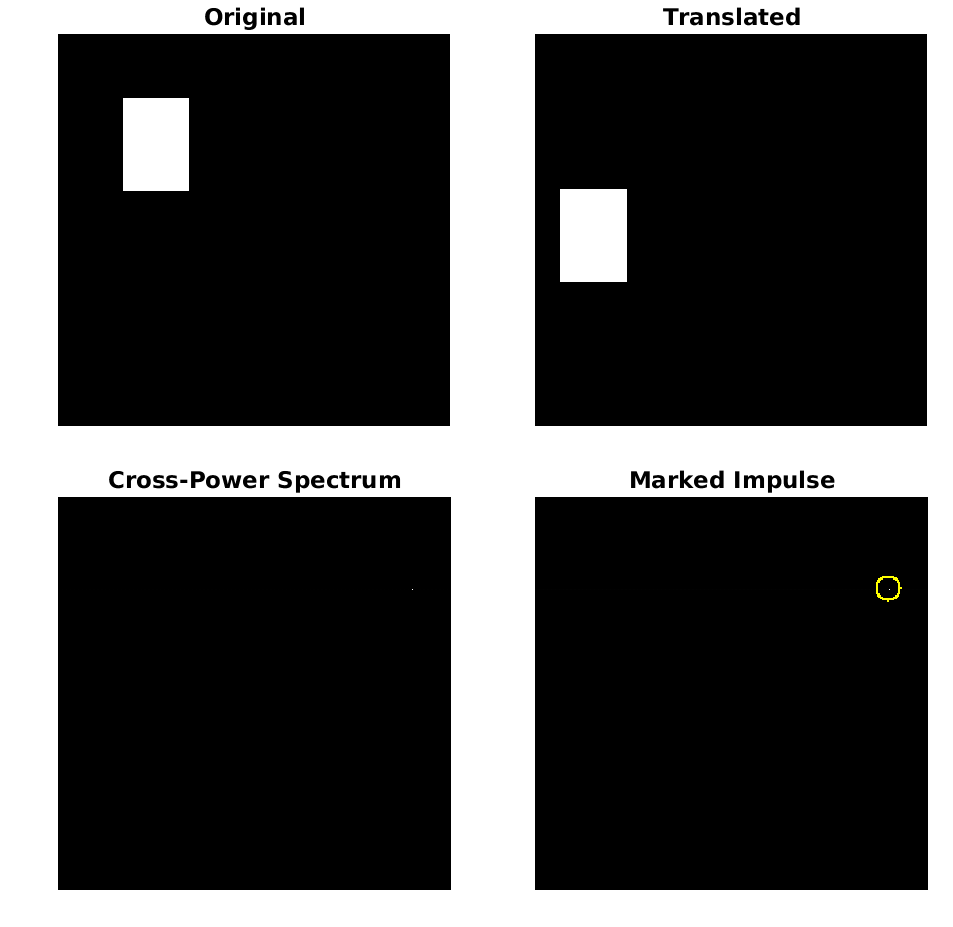
\includegraphics[width=1.34\textwidth]{noiseless.png}
    	\caption{Image Registration}
	    \label{fig:5.1}
    \end{minipage} \\
\end{figure}
\vspace*{40pt}
\newpage
\subsection*{3. Image Registration with noise}
In the noisy case, the translation was obtained at $t_x = -30$ and $t_y = 70$. \\
Below are the corresponding plots. The 4th plot is just the 3rd plot with a marking circle added for better visibility.
\vspace*{65pt}
\begin{figure}[h!]
    \centering
    \renewcommand{\thefigure}{5.2}
    \begin{minipage}[c][1\width]{0.7\textwidth}
    	\hspace*{-0.8in}
    	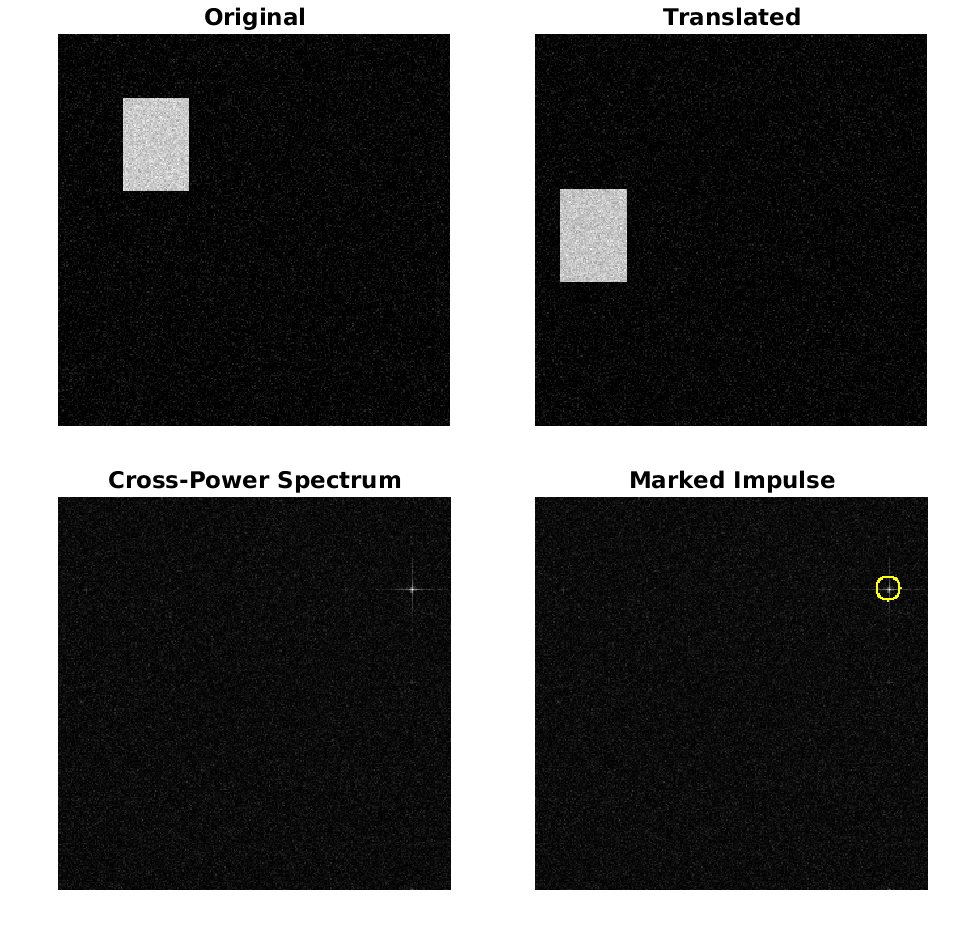
\includegraphics[width=1.34\textwidth]{noisy.png}
    	\caption{Image Registration with Noise}
	    \label{fig:5.2}
    \end{minipage} \\
\end{figure}
\vspace*{40pt}
\newpage
\subsection*{4. Time Complexity Analysis}
For an image of size NxN, the FFT algorithm takes $\mathcal{O}(n^2logn)$ (row-wise/column-wise FFT takes $\mathcal{O}(nlogn)$, and this is done for each of the n rows and columns). The next operation of element wise sum and division take $\mathcal{O}(n^2)$, and the inverse fourier transform again takes $\mathcal{O}(n^2logn)$. \\
Hence the overall time complexity is $\mathcal{O}(n^2logn)$ + $\mathcal{O}(n^2)$ + $\mathcal{O}(n^2logn)$ = $\mathcal{O}(n^2logn)$ \\ \\ 
On the other hand, the pixel wise comparison will take $\mathcal{O}(n^4)$. Basically, we will compute the translated image for every possible translation combination. For a NxN image, there are a total of N$^2$ translation possibilities. For a given translation, the pixelwise similarity computation will again take $\mathcal{O}(n^2)$. \\ Hence the overall time complexity of the brute force algorithm is $\mathcal{O}(n^4)$
\subsection*{5. Correcting Rotation}
The paper has has broken this into two cases - rotation with and without scaling. \\
First we consider rotation without scaling. Let $f_2(x,y)$ be the translated and rotated replica of image $f_1(x,y)$, we have
$$f_2(x,y) = f_1(xcos\theta_0 + ysin\theta_0 - x_0, -xsin\theta_0 + ycos\theta_0 - y_0)$$
We know that a translation changes the phase but not the magnitude. Also, the magnitude is rotation invariant. As mentioned in the paper, using rotation property of the Fourier transform, we get,
$$F_2(\xi ,\eta) = e^{-j2\pi(\xi x_0 + \eta y_0)} M_1(\xi cos\theta_0 + \eta sin\theta_0, -\xi sin\theta_0 + \eta cos\theta_0)$$
Hence the magnitudes M1, M2 are given as follows:
$$M_2(\xi ,\eta) = M_1(\xi cos\theta_0 + \eta sin\theta_0, -\xi sin\theta_0 + \eta cos\theta_0)$$
Since we already know how to compute translation between images, we can convert the above form to polar coordinates, so that the angles are represented in the form of translation.
$$M_2(\rho ,\theta) = M_1(\rho ,\theta-\theta_0)$$
With the algorithm and code used in section 1, we can easily compute the rotation. \\ \\ 
Now, if we want to consider scaling as well, we use logarithmic scale. Following a similar procedure, we get, (from eq 17 in the paper)
$$M_2(\rho ,\theta) = M_1(\rho/a ,\theta-\theta_0)$$
$$M_2(log\rho ,\theta) = M_1(log\rho - loga ,\theta-\theta_0)$$
$$M_2(\xi ,\theta) = M_1(\xi - d ,\theta-\theta_0)$$
where,
$$\xi = log\rho$$
$$d = loga$$
This can be again solved using the formula and algorithm used in section I (for translation).
\subsection*{6. Usage of Code}
\begin{itemize}
\item Simply run the \textbf{myMainScript.m}. This will produce and save all the required plots, and print out the translation values in both the pure and noisy case.
\end{itemize}
\end{document}
